% Functional specification for ProfiSnort
\documentclass[a4paper]{scrreprt}

\usepackage[german]{babel}
\usepackage[utf8]{inputenc}
\usepackage[T1]{fontenc}
\usepackage{ae}
\usepackage[bookmarks,bookmarksnumbered]{hyperref}
\usepackage{csquotes}
\usepackage{longtable}
\usepackage{enumitem, hyperref}
\usepackage{graphicx}

\usepackage[ampersand]{easylist}
\usepackage{xcolor}

\usepackage[toc]{glossaries}

\hypersetup{
    colorlinks,
    linkcolor={red!40!black},
    citecolor={blue!40!black},
    urlcolor={blue!70!black}
}

\makeatletter
\def\namedlabel#1#2{\begingroup
    #2%
    \def\@currentlabel{#2}%
    \phantomsection\label{#1}\endgroup
}
\makeatother

\newcommand{\sppname}{spp\_profinet}
\newcommand{\programname}{Netzwerk.IO}

\makeglossaries


\newacronym
[description={Die grafische Benutzeroberfläche}]
{gui}{GUI}{Graphical User Interface}

\newacronym
[description={Ein Netzwerkprotokoll, das definiert, auf welche Art und Weise Daten zwischen Computern ausgetauscht werden sollen.}]
{tcp}{TCP}{Transmission Control Protocol}

\newacronym
[description={Input und Output}]
{io}{IO}{Input/Output}

\newacronym
[description={System oder Software zur Entdeckung von Netzwerkangriffen}]
{ids}{IDS}{Intrusion Detection System}

\newacronym
[description={Protokoll zur Übermittlung von Daten im Internet}]
{ip}{IP}{Internet Protocol}

\newacronym
[description={Ist eine vom Institute of Electrical and Electronics Engineers (IEEE) entworfene Erweiterung des OSI-Modells.}]
{mac}{MAC}{Media Access Control}

  \newglossaryentry{alert}{
  name=Alert,
  plural=Alerts,
  description={Ein von Snort versendeter Alarm, welcher durch verschieden Regeln abgefangen und verarbeitet werden kann.}
}

  \newglossaryentry{whitelist}{
  name=Whitelist,
  description={is a programmable machine that receives input,
               stores and manipulates data, and provides
               output in a useful format}
}

  \newglossaryentry{blacklist}{
  name=Blacklist,
  description={is a programmable machine that receives input,
               stores and manipulates data, and provides
               output in a useful format}
}

  \newglossaryentry{ethernet}{
  name=ethernet,
  description={is a programmable machine that receives input,
               stores and manipulates data, and provides
               output in a useful format}
}
  \newglossaryentry{headerdaten}{
  name=Headerdaten,
  description={is a programmable machine that receives input,
               stores and manipulates data, and provides
               output in a useful format}
}
  \newglossaryentry{io-supervisor}{
  name=IO\_Supervisor,
  description={is a programmable machine that receives input,
               stores and manipulates data, and provides
               output in a useful format}
}
  \newglossaryentry{linux}{
  name=Linux,
  description={is a programmable machine that receives input,
               stores and manipulates data, and provides
               output in a useful format}
}
  \newglossaryentry{programname}{
  name=\programname,
  description={is a programmable machine that receives input,
               stores and manipulates data, and provides
               output in a useful format}
}
  \newglossaryentry{netzwerkpakete}{
  name=Netzwerkpaket,
  plural=Netzwerkpakete,
  description={is a programmable machine that receives input,
               stores and manipulates data, and provides
               output in a useful format}
}
  \newglossaryentry{profinet}{
  name=PROFINET,
  description={PROFINET (Process Field Network) ist der offene Industrial Ethernet-Standard von Profibus & Profinet International (PI) für die Automatisierung. Profinet nutzt \gls{tcp}/\gls{ip} und IT-Standards, ist Echtzeit-\gls{ethernet}-fähig und ermöglicht die Integration von Feldbus-Systemen.}
}
  \newglossaryentry{profinet-tcp}{
  name=PROFINET TCP,
  description={is a programmable machine that receives input,
               stores and manipulates data, and provides
               output in a useful format}
}
  \newglossaryentry{snort}{
  name=Snort,
  description={Snort ist ein open source \gls{ids} mit realtime Paketanalyse und Paketlogging.}
}
  \newglossaryentry{praeprozessor}{
  name=Präprozessor,
  plural=Präprozessoren,
  description={Ein Präprozessor ist eine art Plugin für \gls{snort}. Er wird nach den Decodern und vor der Rules Engine aufgerufen. Er dient zur fortgeschrittenen Paketverarbeitung wie z.B. Normalisierung oder weiteres Decodieren.}
}
  \newglossaryentry{sppname}{
  name=\sppname,
  description={Der Name des Präprozessors. Der Präprozessor ist dafür zuständig \gls{profinet} \glspl{paket} zu dekodieren.}
}
  \newglossaryentry{x86-64)}{
  name=x86\_64,
  description={64 Bit Architektur}
}



\newglossaryentry{frameid}{
  name=Frame ID,
  description={is a programmable machine that receives input,
               stores and manipulates data, and provides
               output in a useful format}
}

\newglossaryentry{interprocess}{
    name=Interprozesskommunikation,
    description={adfssekjghsalkgtjreah}
}
\newglossaryentry{paket}{
    name=Paket,
    plural=Pakete,
    description={aadsfkdsajgflkahtljewr}
}

\newglossaryentry{log}{
    name=Log,
    plural=Logs,
    description={ageaewhgjreahj}
}

\newglossaryentry{fehlerflag}{
    name=Fehlerflag,
    description={Ein Bit, welches bestimmt ob der Eintrag fehlerhaft ist, oder nicht.}
}

\newglossaryentry{iocontroller}{
    name=IO\_Controller,
    description={}
}

\newglossaryentry{identifyrequest}{
    name=Identify Request,
    description={}
}



\begin{document}

\title{\programname \& \sppname --- Pflichtenheft}
\author{
    Brendl, Julian
    \texttt{ubems@student.kit.edu}
    \and
    Diez, Maximilian
    \texttt{maximilian.diez@student.kit.edu}
    \and
    Giraud, Mark
    \texttt{mark.giraud@student.kit.edu}
    \and
    Hermes, Jan
    \texttt{jan.hermes@student.kit.edu}
    \and
    Höhler, Dimitri
    \texttt{dimitri.hoehler@student.kit.edu}
    \and
    Kiechle, Valentin
    \texttt{unekn@student.kit.edu}
}
\maketitle



\newpage
\tableofcontents
\newpage
\listoffigures

\chapter{Einleitung}
Dieses Dokument dient der genaueren Beschreibung und Dokumentation des Entwurfs zum Visualisierungstool \gls{programname}, dessen Hauptaufgabe die Darstellung des Netzwerkverkehrs eines \gls{profinet}-Systems ist. Des Weiteren wird der im \gls{ids} \gls{snort} eingebaute \gls{praeprozessor} \gls{sppname} und die genaue Funktionsweise der \gls{ipc} zu \gls{programname} erläutert.\newline
\newline


Das Design von \gls{programname} baut auf dem klassischen \gls{mvc} auf und erweitert diesen Entwurf zu einem \gls{mvp} mit zusätzlicher Funktionalität. Das heisst, dass der Controller aufgeteilt wurde in zwei selbständige Packages. Zum Einen das Service-Package. Dabei handelt es sich um entkoppelte, selbstlaufende Routinen, welche fast die gesamte Logik des Programms ausmachen. Sie werden einmal initialisiert und laufen dann solange \gls{programname} läuft. Zum Andern gibt es den Presenter. Dieser erfüllt seine Hauptaufgabe bei Programmstart. Er instanziiert alle für den Programmablauf benötigten Klassen. Außerdem erstellt er sämtiche nötigen Referenzen, übergibt diese, und startet jeden selbständigen Thread wie zum Beispiel die Services. Danach wird der Presenter nicht mehr benötigt.

Der Entwurf von \gls{programname} baut auf das klassische \gls{mvc} Design auf, welches bereits im Pflichtenheft präsentiert wurde (siehe Abbildung~\ref{fig:old_arch_diagram}). Das erweiterte \gls{mvc} Modell in Abbildung~\ref{fig:arch_diagram} zeigt, dass der Aufbau sich um folgende Bestandteile

MODEL:
Wie im traditionellen \gls{mvc} Muster dient das Model ausschließlich zur Speicherung von Daten in geeigneten Datenstrukturen. Im Fall von \gls{programname} umfasst dies den Graphen (siehe Kapitel~\ref{subsubsec:graph}.) und die Programmeinstellungen.

VIEW:
Auch der View unterscheidet sich kaum von der ursprünglichen Funktionalität. Er dient weiterhin dazu, dem Benutzer eine Plattform zur Interaktion mit dem Programm zu bieten. Ein wesentlicher Unterschied zum ursprünglichen Aufbau ist hierbei jedoch, dass der View nur spezifische Interaktionen (siehe INTERACTIONS) kennt und ausführen kann. Wobei der View keine Kenntnis über die hinter der Aktion stehende Logik hat.

INTERACTIONS:
Wie bereits im vorherigen Absatz beschrieben, dienen Interaktionen dem View als 

COMMANDS:
Kommandos sind neben dem SERVICE Package die eigentlichen 

PRESENTER:
Im Presenter wird die gesamte Aufbauarbeit geleistet. Kommandos werden mit bestimmten Interaktionen gelinkt, grafische Oberflächen werden instanziiert und vorbereitet und das Modell.
Zusätzlich kümmert sich der Presenter darum, dass sämtliche Service Routinen gestartet werden 


Der Presenter ist dafür verantwortlich, dass sämtliche Klassen instanziiert werden 

Wie  in 


\begin{figure}[H]
  \centering
  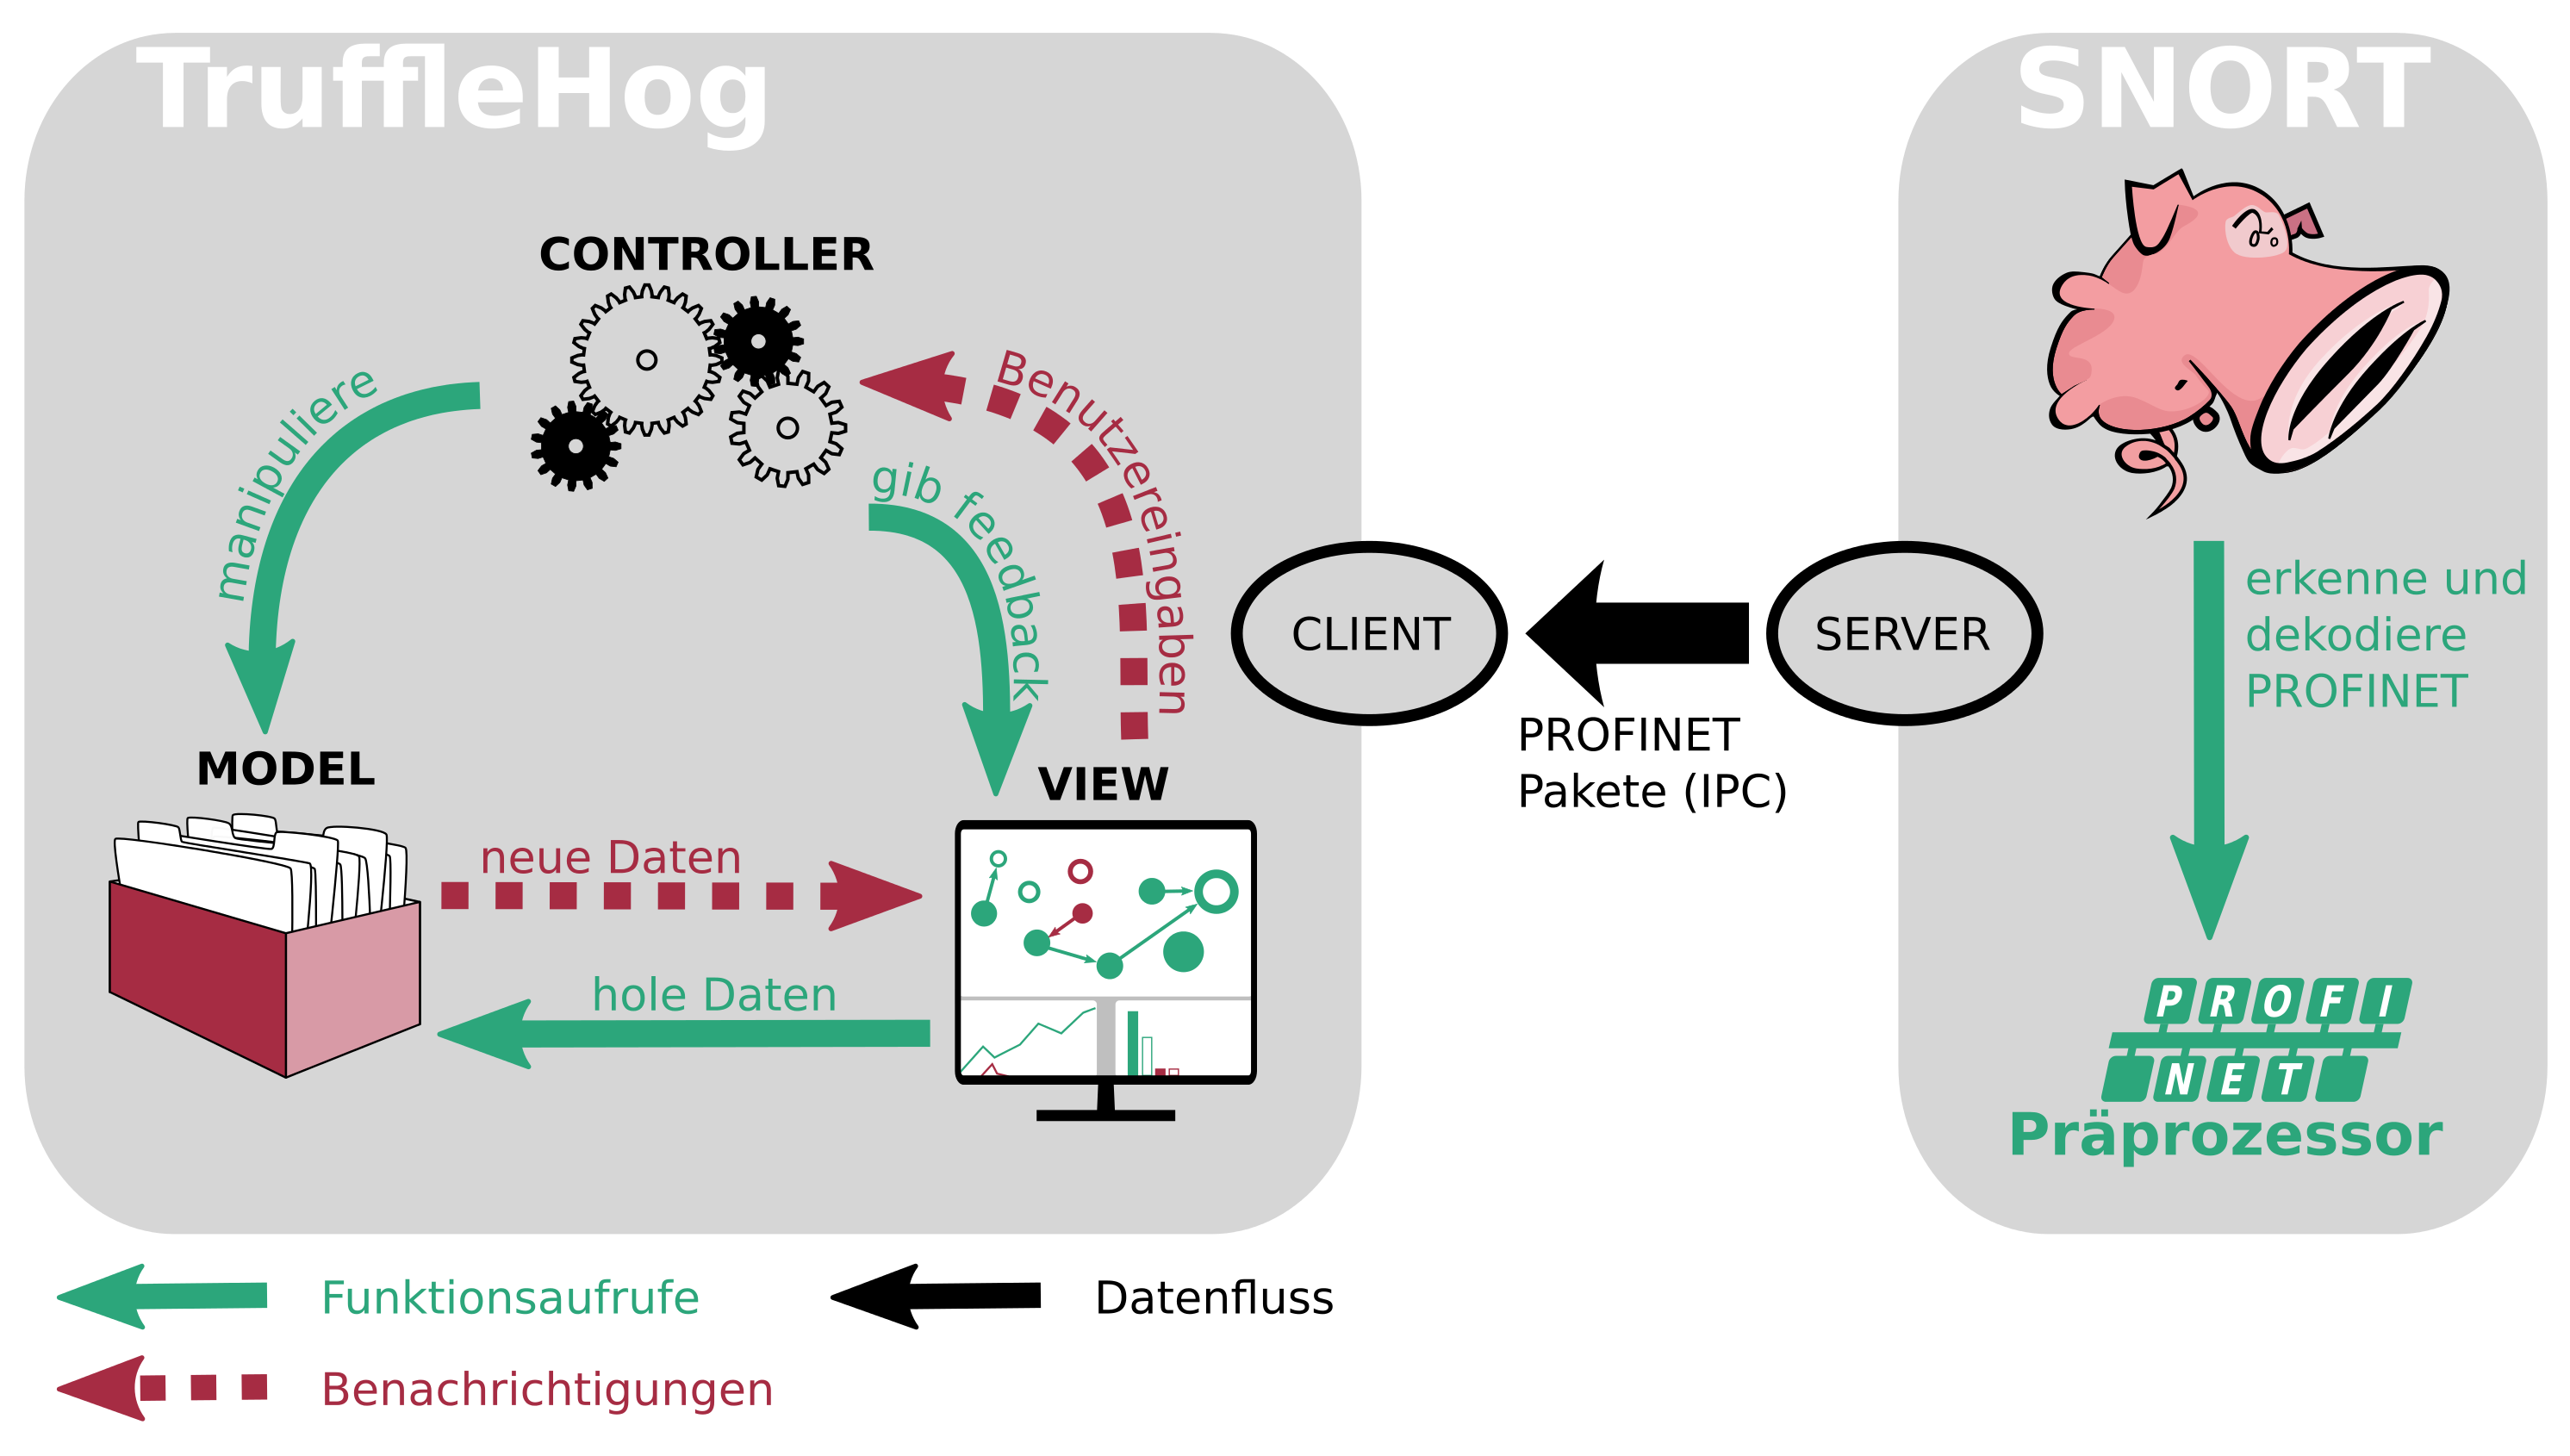
\includegraphics[width=0.8\textwidth]{../diagramimages/praesentationsmodel.png}
  \caption[Urspr''ungliche Architektur''ubersicht]{Urspr''ungliche Architektur''ubersicht}
  \medskip
  Ursprünglicher Aufbau der Programme aus dem Pflichtenheft
\end{figure} 

\begin{figure}[H]
  \centering
  \includegraphics[width=0.8\textwidth]{../diagramimages/arch_diagram_mvp_single.pdf}
  \caption[Erweiterte Architekturu''bersicht]{Erweiterte Architekturu''bersicht}
  \medskip
  Erweiterte Strukturierung des Programms nach dem \gls{mvp}
\end{figure} 

\chapter{Zielbestimmung}

\gls{programname} und \gls{sppname} sollen eine Möglichkeit schaffen, das \gls{ids} \gls{snort} auch mit \gls{profinet} verwenden zu können.
Hierbei soll \gls{programname} eine übersichtliche Darstellung der Beziehungen und Datenflüsse des überwachten Netzwerkes bieten.

\section{Musskriterien}

\subsection{\gls{sppname} (Snort-Präprozessor)}

\begin{itemize}
\item Der \gls{praeprozessor} muss \gls{ethernet} \gls{profinet} Pakete erkennen und dekodieren können.

\item Der \gls{praeprozessor} muss ein Ausgabeinterface bereitstellen damit \gls{programname} die dekodierten Paketdaten empfangen und weiterverarbeiten kann.

\item Der \gls{praeprozessor} muss die \gls{profinet} \gls{headerdaten} zusammenfassen und an \gls{programname} weitergeben.
\end{itemize}

\subsection{\gls{programname} (Analyseprogramm)}

\begin{itemize}
\item Das Analyseprogramm muss eine grafische Oberfläche mit folgenden Funktionen bieten:

	\begin{itemize}
    \item Übersichtliched Darstellung der Kommunikationsbeziehungen eines Netzwerks mithilfe eines Graphen.

    \item Netzwerkteilnehmer werden im Graphen als Knoten dargestellt, Kommunikationswege als Kanten.

    \item Möglichkeit zur zusätzlichen Darstellung von detaillierten Informationen (z.B. Paketdurchsatz, letzte Aktivität).

    \item Vergößern und Verkleinern des Graphen (Zoom).

    \item Es gibt ein Einstellungsmenü, welches dem Nutzer ermöglicht grundlegende Einstellungen (bspw. Sprachwahl, Farbwahl) vorzunehmen.
    \end{itemize}

\item Es gibt eine Möglichkeit Bestimmte Subnetze auf eine \gls{blacklist} bzw. \gls{whitelist} zu setzen.

\item Durch White- oder Blacklist als legal bzw. illegal markierte Kommunikation muss unterschiedlich dargestellt werden.

\item \gls{programname} zeichnet Netzwerkkommunikation in \glspl{log} auf.

\item Die Maximalgröße aufzuzeichnender \glspl{log} kann im Einstellungsmenü festgelegt werden.

\item Das Analyseprogramm muss die Möglichkeit zur Datenhaltung und möglichen späteren Auswertung bieten.

\item Das Programm funktioniert eigenständig und hat möglichst wenige Abhängigkeiten.

\item Der Paketdurchsatz kann in einem Detailfenster in textueller Form eingesehen werden.

\item Die Bezeichnung der \gls{frameid} eines Paketes kann, soweit bekannt, im Graph dargestellt werden.

\end{itemize}

\section{Kannkritierien}

\subsection{\gls{sppname}}

\begin{itemize}

\item Der \gls{praeprozessor} kann die dekodierten Pakete \gls{snort} zur Verfügung stellen, damit sie dort weiterverarbeitet werden können.

\item Der \gls{praeprozessor} ist in der Lage andere Protokollarten die \gls{profinet} verwendet (z.B. \gls{tcp}, \gls{udp}, \gls{lldp}) zur Weiterverarbeitung an \gls{programname} weiterzugeben.

\item Der \gls{praeprozessor} kann \gls{snort} \glspl{alert} auslösen. Die Rule Engine von \gls{snort} wird dabei nicht verwendet.
\end{itemize}

\subsection{\gls{programname}}

\begin{itemize}
\item Das Analysetool kann dem Nutzer grafische Statistiken des bisher stattgefundenen Netzwerkverkehrs anzeigen.

\item Das Analysetool kann von \gls{snort} ausgelöste \glspl{alert} im Graph darstellen.

\item Die Richtung des Kommunikationsflusses kann im Graphen dargestellt werden.

\item Der Paketdurchsatz kann im Graph visuell gekennzeichnet werden (z.B. Farbe der Kante).

\item Dem Benutzer wird ermöglicht, Knoten anhand von Kriterien zu filtern (z.B. Adresse, Name).

\item Der Benutzer hat die Möglichkeit über ein Menü geeignete Algorithmen zur Darstellung des Graphen auszuwählen.
\end{itemize}

\section{Abgrenzungskriterien}

\subsection{\gls{sppname}}
\begin{itemize}
\item Der \gls{praeprozessor} soll nicht die Arbeit von \gls{snort} und dem Analysetool übernehmen.

\item Der \gls{praeprozessor} soll nur dekodieren und nicht analysieren.

\end{itemize}

\subsection{\gls{programname}}
\begin{itemize}

\item \gls{programname} bietet keinen aktiven Schutz vor Angriffen, sondern zeigt solche nur an (Das Programm dient lediglich der Analyse und Visualisierung des Netzwerkverkehrs).

\item Die Graphalgorithmen  werden einer Bibliothek entnommen und nicht selbst entwickelt.

\item Die \gls{gui} wird nicht von Grund auf neu entwickelt, sondern verwendet Bibliotheken um die Entwicklung zu erleichtern.

\end{itemize}


\chapter{Produkteinsatz}

\section{Anwendungsbereiche}
\gls{programname} soll zur Visualisierung von industriellen Netzwerken und zur potentiellen Gefahrenerkennung eingesetzt werden.

\section{Zielgruppen}
Institute und Forschungsgruppen, die sich mit Sicherheit in der Industrie und der Visualisierung von komplexen Netzen beschäftigen. Das Programm richtet sich auch an Menschen mit Grundverständnis der IT-Sicherheit, die sich mit dem Thema vertraut machen möchten.\newline\newline
Industrielle Anlagen, die eine laufende Übersicht ihres Datenverkehrs sehen möchten. Man könnte sich dabei vorstellen, dass \gls{programname} dabei die Funktion einer Überwachungskamera übernimmt, da sich die Netzwerkaktivität in Echtzeit überwachen lässt und zusätzlich die Möglichkeit besteht Aktivitäten aus der Vergangenheit anhand aufgezeichneter \glspl{log} zurück zu verfolgen.

\section{Betriebsbedingungen}
Das Programm ist für eine industrielle Betriebsumgebung mit \gls{profinet} als Kommunikationsprotokoll ausgelegt. Es ist hauptsächlich für \gls{linux} Betriebssysteme ausgelegt und läuft nur auf diesen garantiert.


\chapter{Produktumgebung}

\section{Software}
Das Produkt wird zusammen mit Snort 2.9.7 ausgeliefert. Es läuft standardmäßig nur auf Linux, kann aber unter Umständen auf Windows kompiliert werden. Als Architektur ist x86(\_64) vorgesehen.

\section{Hardware}
Um optimale Ergebnisse bei der Analyse eines Netzwerks zu erhalten, ist ein zentraler Anschlusspunkt in das Netzwerk nötig.
Netzwerk.IO ist für eine x86\_64 Architektur entwickelt.

\chapter{Funktionale Anforderungen}

\renewcommand{\arraystretch}{2}
\section{\sppname}
\begin{tabular}{lp{0.9\linewidth}}

FA10: & \textit{Erkennung fehlerhafter Pakete: }Der Präprozessor muss fehlerhafte Pakete erkennen und diese als solche markieren können, bevor sie an das Analysetool weitergereicht werden. \\

FA20: & \textit{Erkennen von PROFINET Paketen: }Der Präprozessor muss PROFINET Pakete erkennen können. \\

FA30: & \textit{Dekodieren von PROFINET Pakten: }Der Präprozessor muss die erkannten Pakete dekodieren können. \\

FA40: & \textit{Unterscheiden der verschiedenen Frame IDs: }Der Präprozessor muss die verschiedenen von PROFINET spezifizierten Frame IDs unterscheiden können.\\

FA50: & \textit{Output Kanal zu \programname: }Es muss eine Interprozesskommunikation für die Weitergabe der dekodierten Daten möglich sein.\\

FA60: & \textit{Starten von \programname: }Wenn in der .config Datei eingestellt, startet sich \programname automatisch. Diese Option ist standardmäßig deaktiviert.\\

FA70: & \textit{Ausgabeschnittstelle: }\sppname muss eine einheitliche Schnittstelle zum Übertragen der Daten an \programname verwenden. Diese Schnittstelle muss prinzipiell auf andere Protokolle erweiterbar sein.\\

\end{tabular}

\section{\programname}
\subsection{Funktionalität}

\begin{longtable}{lp{0.9\linewidth}}

FA90: & \textit{Starten von Snort: }Wenn Snort noch nicht läuft wird Snort automatisch gestartet. \\

FA100: & \textit{\sppname anschalten: }Wenn \sppname in der Snort Konfiguration deaktiviert ist, wird der Benutzer gefragt ob er dies aktivieren möchte. Falls der Benutzer \sppname nicht aktiviert, beendet sich \programname. \\

FA110: & \textit{Snort läuft aber \sppname ist deaktiviert: }Falls Snort schon läuft aber \sppname deaktiviert ist, wird dem Benutzer die Wahl gestellt das Plugin zu aktivieren oder \programname zu deaktivieren. Falls das Plugin aktiviert werden soll, wird Snort mit dem reload Befehl neu geladen.\\

FA120: & \textit{Empfangen von Paketinformationen: }\programname muss Paketinformationen empfangen können, die in dem in FA70 genannten Interface entsprechen. \\

FA130: & \textit{Erkennen neuer Netzwerkteilnehmer: }Das Programm erkennt neue Netzwerkteilnehmer und erstellt einen neuen Knoten. Zusätzlich wird eine kurze Warnung ausgegeben, die nach kurzer Zeit verschwindet. \\

FA140: & \textit{Erkennen von Gerätenamen: }Das Analysetool soll Gerätenamen, falls vorhanden, erkennen und dem entsprechenden Knoten hinzufügen. \\

FA150: & \textit{Kennzeichnen illegaler Knoten: }Ein Knoten der ein Gerät aus einem illegalen Adressraum repräsentiert oder eine unbekannte/unerwünschte/illegale Identität hat werden für den Nutzer auffällig gekennzeichnet. \\

FA160: & \textit{Kennzeichnen illegaler Kanten: }Kanten, die eingehende und ausgehende Kommunikation eines illegalen Knotens repräsentieren werden für den Nutzer auffällig gekennzeichnet. \\

FA170: & \textit{Erkennen der Kommunikationswege: }Das Programm muss basierend auf Adressen/Gerätenamen einen Kommunikationsgraphen erstellen können. \\

FA180: & \textit{Paketaustausch Statistik: }Das Programm muss berechnen können, wie viele Pakete einzelne Knoten pro Sekunde senden bzw. Empfangen. Diese Information muss in dem Fenster zur Detaillierten Knotenstatistik darstellbar sein. \\

FA190: & \textit{Gesamtzahl der Pakete: }Das Programm muss die gesamte Zahl der empfangenen und gesendeten Pakete in dem Fenster zur Detaillierten Knotenstatistik darstellen können. \\

FA210: & \textit{Darstellung des Paketvolumens: }Das Paketvolumen der Pakete ist im Graph visuell darstellbar. Diese Darstellung kann in den Einstellungen der Übersicht halber deaktiviert werden. \\

FA220: & \textit{Zeichnen des Graphen: }Der Graph kann mittels verschiedener Graphalgorithmen gezeichnet werden. \\

FA230: & \textit{Sprachwechsel: }Das Programm soll so gebaut sein, dass ein einfacher Sprachwechsel der GUI möglich ist. \\

FA240: & \textit{Timeoutbenachrichtigung: }Wenn ein IO\_Controller ein Identify Request sendet und ein Timeout stattfindet wird der Nutzer grafisch darüber in Kenntnis gesetzt. \\

FA250: & \textit{Kantenunterschied: }Die Unterschiedlichen PROFINET Protokollen werden durch Labels oder Farben voneinander unterscheidbar sein. \\

FA260: & \textit{Logging: }Das Programm erstellt ein Log aller Pakete mit kritischen Informationen und kann dieses auf Benutzerwunsch als Textdatei ausgeben. \\

FA270: & \textit{Spezifisches Logging: }Das Programm erstellt spezifische Logdateien zu einzelnen Knoten mit von diesem Knoten gesendeten/empfangenen Paketen. \\

FA280: & \textit{Fehlerhafte Pakete: }Von \sppname als fehlerhaft erkannte Pakete werden als fehlerhaft ins Log übernommen.

\end{longtable}

\subsection{Optionale Funktionalität}
\begin{tabular}{lp{0.9\linewidth}}

FA290: & \textit{Rückverfolgung: }Der Nutzer kann den zeitlichen Ablauf grafisch zurückverfolgen (wie ein Video) und sämtliche Kommunikationswege erneut abspielen. \\

FA300: & \textit{Kennzeichnen inaktiver Knoten: }Knoten werden nach einer im Einstellungsmenü spezifizierten Zeit als inaktiv gekennzeichnet, wenn sie in dieser Zeit keine Pakete empfangen oder gesendet haben. \\

FA310: & \textit{Abgrenzen gefilterter Knoten: }Alle Knoten, die nicht den Filteroptionen genügen, werden optisch vom Rest des Graphen getrennt. \\

\end{tabular}

\subsection{Datenhaltung}

\begin{tabular}{lp{0.9\linewidth}}

FA320: & \textit{Speichern des Datenverkehrs: }Der Datenverkehr wird in einer Datenbank gespeichert. \\

FA330: & \textit{Kategorisierung der Daten: }Die Daten werden nach den verschiedenen Kommunikationstypen kategorisiert. \\

FA340: & \textit{Datenausgabe: }Auf Anforderungen des Benutzers müssen Daten ausgelesen und ausgegeben werden. \\

FA350: & \textit{Zeitraum der Datenspeicherung: }Der Zeitraum über den die Daten gespeichert werden sollen kann in den Einstellungen festgelegt werden. \\

\end{tabular}

\subsection{Benutzerinteraktion}

\begin{tabular}{lp{0.9\linewidth}}

FA360: & \textit{Speichern der Einstellungen: }Das Programm speichert nach Änderungen des Nutzers automatisch bzw. nach klick auf den Speichern Knopf die neuen Einstellungen. \\

FA 370: & \textit{Fehlerhafte Nutzereingaben: }Die Nutzereingaben im Einstellungsmenü und Filtermenü werden auf Fehler überprüft. Bei Fehlern wird der Benutzer zur neuen Eingabe aufgefordert und der vorherige Wert nicht verändert. \\

FA380: & \textit{Skalierung des Graphen: }Der Benutzer ist in der Lage über das Scrollrad die Skalierung des Graphen zu verändern. \\

FA390: & \textit{Detaillierte Information zu Knoten: }Ein Overlay mit detaillierten Informationen wird bei Klick auf einen Knoten dargestellt. \\

FA400: & \textit{Generelle Informationen: }In einem Overlay werden generelle Informationen über den Graph angezeigt. \\

FA410: & \textit{Hover statt Klick: }Hovern erfüllt im Graph die selben Funktionen wie klicken. Zusätzlich zum aktuellen Knoten werden zum Vergleich Informationen des aktuell gehoverten Knotens angezeigt. \\

FA420: & \textit{Blacklist: }Der Nutzer hat die Möglichkeit, bestimmte MAC- und IP Adressräume sowie Gerätenamen als illegal zu markieren. \\

FA425: & \textit{Whitelist: }Der Nutzer hat die Möglichkeit, bestimmte MAC- und IP Adressräume sowie Gerätenamen als legal zu markieren. \\

FA427: & \textit{Whitelist/Blacklist aktivieren: }Der Nutzer kann über das Einstellungsmenü wählen, welche Listen verwendet werden sollen. \\

\end{tabular}

\subsection{Optionale Benutzerinteraktion}

\begin{tabular}{lp{0.9\linewidth}}

FA430: & \textit{Statistiken zu Knoten: }Ein Overlay mit zeitlichen Statistiken wird bei Klick auf einen Knoten angezeigt. \\

FA440: & \textit{Filtereinstellungen: }Die Filtereinstellungen können im Einstellungsmenü angepasst werden. \\

FA450: & \textit{Filteroptionen: }Die Knoten können nach IP, MAC Adresse,, Netzwerkaktivität oder Gerätenamen gefiltert werden. \\

FA460: & \textit{Filter deaktivieren/reaktivieren: }Es gibt einen Hotkey und eine Option im Filterfenster zum aktivieren oder deaktivieren von Filtern. \\

FA470: & \textit{IO\_Supervisor festlegen: }Der Nutzer kann Geräte eindeutlig spezifizieren, die das Programm als IO Supervisor markiert \\ % TODO (wie) wollen wir das im graphen repräsentieren?

FA480: & \textit{Verbindungsrichtung: }Wenn mindestens x\% (standardmäßig 90\%, konfigurierbar) der Pakete aus einer Richtung kommen, werden Verbindungen im Graph gerichtet angezeigt. \\

FA490: & \textit{Graphdarstellungsalgorithmen: }Die Graphdarstellungsalgorithmen können über das Einstellungsmenü ausgewählt/geändert werden. \\

FA500: & \textit{Kategorisierung: }Einzelne Knoten können im Graphen als unwichtig eingestuft werden, um diese visuell weniger hervorzuheben. \\
\end{tabular} 

\chapter{Nichtfunktionale Anforderungen}
% this is a test comment try 2


\chapter{Produktdaten}


\begin{itemize}
  \item \gls{programname} hält einen \gls{log} von vergangenen, bearbeiteten \glspl{paket} eines gewissen Zeitraums in Form eines Datenbestands. Gespeichert werden folgende Daten:

  \begin{itemize}
    \item Der Zeitpunkt des Eintreffens der Pakete.
    \item Die Headerdaten der Pakete.
    \end{itemize}
  \item Im Fall eines \glspl{alert} wird dieser in einer Logdatei gespeichert.
  \item Seit Programmstart gesetzte Einstellungen werden gespeichert.
\end{itemize}

\chapter{Globale Testfälle}

\section{Funktionstests zu prüfen}

\begin{description}[style=multiline, leftmargin=4cm, labelwidth=4cm]
  \item[\namedlabel{start}{Programm starten}] Der Nutzer startet \programname, wird gefragt ob er Snort mit dem Präprozessor neu starten will, da dieser noch nicht läuft, stellt im Einstellungsmenü die Länge des Kommunikationslogs auf 10 Minuten.
  \item[\namedlabel{addNetNode}{Kommunikationsteilnehmer hinzufügen}] Ein Kommunikationsteilnehmer wird zum Netzwerk hinzugefügt indem er anfängt PROFINET-Pakete zu senden. Er erscheint auf der GUI, Gerätename/IP-Adresse/MAC-Adresse ist direkt sichtbar. Der Nutzer lässt sich mit einem Klick die Knoten-Details anzeigen.
  \item[\namedlabel{normalWatch}{Normale Netzwerküberwachung}] Es kommuniziert ein Beispielnetzwerk von 5 Teilnehmern über PROFINET, in der GUI baut sich ein Graph selbständig auf und zeigt jeden Kommunikationsteilnehmer sowie die zugehörigen Verbindungen an. Alle Kommunikationswege werden als legal gekennzeichnet. Der Nutzer lässt sich die Log-Dateien der letzten 10 Minuten anzeigen.
  \item[\namedlabel{guiDisplay}{Korrekte GUI Darstellung}] Ein Paketsender sendet den gleichen Datenverkehr zu einem zweiten, neuen Empfänger, die GUI zeigt dies an. Weiter sind die Logs der Verbindungen, welche in der GUI durch den Nutzer abgerufen werden, bis auf die Adressen identisch zwischen beiden Empfängern.
  \item[\namedlabel{filter}{Filter anwenden}] Der Nutzer stellt im Filtereinstellungsmenü den Namensfilter ein und lässt sich alle Knoten mit Unternamen “Haribo” markieren. \\Die GUI graut alle anderen Knoten aus.
  \item[\namedlabel{guiChanging}{Graph verändern}] Der Nutzer skaliert den Graphen klein(zoomt raus). \\Der Nutzer wählt einen alternativen Graph-Darstellungsalgorithmus.
  \item[\namedlabel{inactive}{Netzteilnehmer wird inaktiv}] Ein Paketsender wird aus dem Netz entfernt (hört auf zu senden), er wird nach zuvor vom Nutzer eingestellten 5 Sekunden als inaktiv markiert.
  \item[\namedlabel{errpak}{Fehlerhaftes Paket}] Ein fehlerhaftes Paket wird von einem Paketsender gesendet, der Nutzer lässt sich die Log-Dateien anzeigen und sieht das als fehlerhaft markierte Paket.
  \item[\namedlabel{blacklist}{Blacklist}] Ein Angreifer mit Blacklist-Adresse im Netzwerks löst Illegale-Kommunikation-Alarm aus und erscheint auf der GUI inklusive Warnung für den Nutzer. Die Kommunikation wird als illegal angezeigt.
  \item[\namedlabel{inactiveBlacklist}{Inaktiver geblacklisteter Teilnehmer}] Nach \ref{blacklist} hört der Angreifer auf zu kommunizieren. Daraufhin wird er als inaktiv aber weiterhin als Angreifer angezeigt. Seine Logs werden separat gespeichert und sind für den Nutzer lesbar.
  \item[\namedlabel{Exit}{Exit}] \programname (Programm) beenden.
  \item[\namedlabel{Absturz}{Absturz}] \programname-Prozess wird terminiert. Es muss sichergestellt sein, dass keine Dateninkonsistenzen auftreten.
\end{description}

\section{Testszenarien}

\begin{itemize}
  \item \ref{start}, \ref{Exit}
  \item \ref{start}, \ref{addNetNode}, \ref{Exit}
  \item \ref{start}, \ref{normalWatch}, \ref{Exit}
  \item \ref{start}, \ref{normalWatch}, \ref{guiDisplay}, \ref{Exit}
  \item \ref{start}, \ref{filter}, \ref{Exit}
  \item \ref{start}, \ref{normalWatch}, \ref{guiChanging}, \ref{Exit}
  \item \ref{start}, \ref{normalWatch}, \ref{inactive}, \ref{Exit}
  \item \ref{start}, \ref{addNetNode}, \ref{errpak}, \ref{Exit}
  \item \ref{start}, \ref{normalWatch}, \ref{blacklist}, \ref{inactiveBlacklist}, \ref{Exit}
  \item \ref{start}, \ref{normalWatch}, \ref{Absturz}
  \item \ref{start}, \ref{normalWatch}, \ref{filter}, \ref{Absturz}, \ref{start}, \ref{addNetNode}, \ref{filter}, \ref{errpak}, \ref{Absturz}, \ref{start}, \ref{normalWatch}, \ref{Exit}
\end{itemize}


\chapter{Systemmodelle}



\section{Szenarien}

\subsubsection*{Akteure}

\begin{tabular}{lp{0.9\linewidth}}

Tom & Der Benutzer des Programms \programname. \\

Udo & Der Angreifer des Firmennetzwerkes. \\

Insekura & Die Firma dessen Geräte ProfiNet zur internen Kommunikation verwenden. \\

\programname & Die Software zur Beobachtung der Netzwerkkommunikation.\\

\end{tabular}

\subsection{Szenario 1: Hinzufügen von erlaubten Adressen}

Tom's Firma Insekura nutzt das industrielle Protokoll ProfiNet für die Kommunikation zwischen den Geräten des Systems. Bisher hat Tom keine Möglichkeit gehabt den Netzwerkverkehr zwischen den Drehmaschinen zu kontrollieren. Während des laufenden Betriebs greift der ehemalige Mitarbeiter Udo unbeobachtet auf den Maschinenablauf zu und verursacht dadurch eine Werkzeugkollision. Der materielle Schaden für die Firma ist groß, ein Mitarbeiter wurde leicht verletzt. Zudem kann Tom den Ablauf der Kommunikation und damit die Ursache des Schadens nicht zurückverfolgen.

In der Hoffnung Unfälle und Attacken solcher Art in Zukunft vermeiden zu können, installiert er die freie Software \programname und lässt sie auf einem gut sichtbaren Bildschirm in seinem Büro dauerhaft in Betrieb. Auf dem Display sieht er sämtliche \textbf{Geräte als Knoten} eines Graphen und kann die \textbf{Kommunikationswege zwischen Geräten und Controllern durch gerichtete Kanten} gut verfolgen. In den Einstellungen von \programname \textbf{fügt er den Adressraum des Firmennetzes zu den erlaubten Kommunikationsadressen hinzu}.

\subsection{Szenario 2: Echtzeit Beobachtung von Angriffen}

Im Laufe der nächsten Tage startet Udo einen weiteren Versuch seiner alten Firma zu schaden. Letztes Mal hat das wunderbar funktioniert, keiner konnte seine fremde Adresse identifizieren und er hatte uneingeschränkte Möglichkeiten falsche Daten an die Drehmaschinen zu übermitteln.

Während sich Udo den Zugang auf das System verschafft, sitzt Tom in seinem Büro und hat seinen Blick gerade auf den Bildschirm mit dem laufenden \programname gerichtet. Er sieht wie ein roter Knoten auf dem Bildschirm erscheint und mit einer der Drehmaschinen beginnt zu kommunizieren. Die Kommunikationskante ist auch rot gekennzeichnet. Sofort eilt Tom zur Tür und drückt auf den Notfall Ausschalter des Systems. Schlimmeres konnte verhindert werden.

\subsection{Szenario 3: Auslesen von Log Dateien}

Tom öffnet die log Datei des roten Knotens, der den Angriff gestartet hat und kann dadurch zurückverfolgen wer sich unerlaubten Zugriff auf das Firmennetzwerk verschafft hat. Udo steht eine große Schadensersatzklage bevor.


\section{Anwendungsfälle}

\subsection{Markieren von Adressen und Namen}

\begin{tabular}{lp{0.9\linewidth}}

\textbf{Name} & Anpassen erlaubter/unerlaubter Adressen und Namen \\

\textbf{Teilnehmender Akteur} & Benutzer \\

\textbf{Eingangsbedingung} &
				\begin{minipage}[t]{\linewidth}
				\begin{itemize}[nosep,after=\strut,leftmargin=10pt]
				
				\item \programname und Snort mit \sppname sind in Betrieb

				\end{itemize}
				\end{minipage} \\
\textbf{Ereignisfluss} &
				\begin{minipage}[t]{\linewidth}
				\begin{itemize}[nosep,after=\strut,leftmargin=10pt]

				\item Benutzer navigiert ins Einstellungsmenü
				\item Benutzer passt die gewünschte Liste an
				\item Benutzer bestätigt Änderungen
				
				\end{itemize}
				\end{minipage} \\

\end{tabular}

\subsection{Netzwerkaktivität beoboachten}

\begin{tabular}{lp{0.9\linewidth}}
\textbf{Name} & Netzwerkaktivität beobachten \\

\textbf{Teilnehmender Akteur} & Benutzer \\

\textbf{Eingangsbedingung} &
				\begin{minipage}[t]{\linewidth}
				\begin{itemize}[nosep,after=\strut,leftmargin=10pt]
				
				\item \programname und Snort mit \sppname sind in Betrieb
				\item Aktiver Datenverkehr zwischen Geräten des Netzwerkes

				\end{itemize}
				\end{minipage} \\
\textbf{Ereignisfluss} &
				\begin{minipage}[t]{\linewidth}
				\begin{itemize}[nosep,after=\strut,leftmargin=10pt]

				\item Benutzer beobachtet und interagiert mit der Benutzeroberfläche
				\end{itemize}
				\end{minipage} \\

\end{tabular}

\subsection{Graph skalieren}

\begin{tabular}{lp{0.9\linewidth}}
\textbf{Name} & Graph skalieren \\

\textbf{Teilnehmender Akteur} & Benutzer \\

\textbf{Eingangsbedingung} &
				\begin{minipage}[t]{\linewidth}
				\begin{itemize}[nosep,after=\strut,leftmargin=10pt]
				
				\item \programname und Snort mit \sppname sind in Betrieb
				\item Aktiver Datenverkehr zwischen Geräten des Netzwerkes

				\end{itemize}
				\end{minipage} \\
\textbf{Ereignisfluss} &
				\begin{minipage}[t]{\linewidth}
				\begin{itemize}[nosep,after=\strut,leftmargin=10pt]
				\item Benutzer dreht das Mausrad
				\end{itemize}
				\end{minipage} \\
\end{tabular}

\subsection{Einstellungen speichern}

\begin{tabular}{lp{0.9\linewidth}}
\textbf{Name} & Graph skalieren \\

\textbf{Teilnehmender Akteur} & Benutzer \\

\textbf{Eingangsbedingung} &
				\begin{minipage}[t]{\linewidth}
				\begin{itemize}[nosep,after=\strut,leftmargin=10pt]
				
				\item \programname und Snort mit \sppname sind in Betrieb

				\end{itemize}
				\end{minipage} \\
\textbf{Ereignisfluss} &
				\begin{minipage}[t]{\linewidth}
				\begin{itemize}[nosep,after=\strut,leftmargin=10pt]
				\item Benutzer navigiert ins Einstellungsmenü
				\item Benutzer klickt auf den "Einstellungen speichern" Eintrag
				\end{itemize}
				\end{minipage} \\
\end{tabular}

\subsection{Programm beenden}

\begin{tabular}{lp{0.9\linewidth}}
\textbf{Name} & Graph skalieren \\

\textbf{Teilnehmender Akteur} & Benutzer \\

\textbf{Eingangsbedingung} &
				\begin{minipage}[t]{\linewidth}
				\begin{itemize}[nosep,after=\strut,leftmargin=10pt]
				
				\item \programname und Snort mit \sppname sind in Betrieb

				\end{itemize}
				\end{minipage} \\
\textbf{Ereignisfluss} &
				\begin{minipage}[t]{\linewidth}
				\begin{itemize}[nosep,after=\strut,leftmargin=10pt]
				\item Benutzer navigiert ins File Menü
				\item Benutzer klickt auf den Eintrag "Exit"
				\item Benutzer wird gefragt ob Einstellungen gespeichert werden sollen
				\item Programm wird beendet
				\end{itemize}
				\end{minipage} \\
\end{tabular}


\pagebreak
\subsection*{Anwendungsfalldiagramm - Benutzerinteraktion}


\begin{figure}[h!]
    \centering
    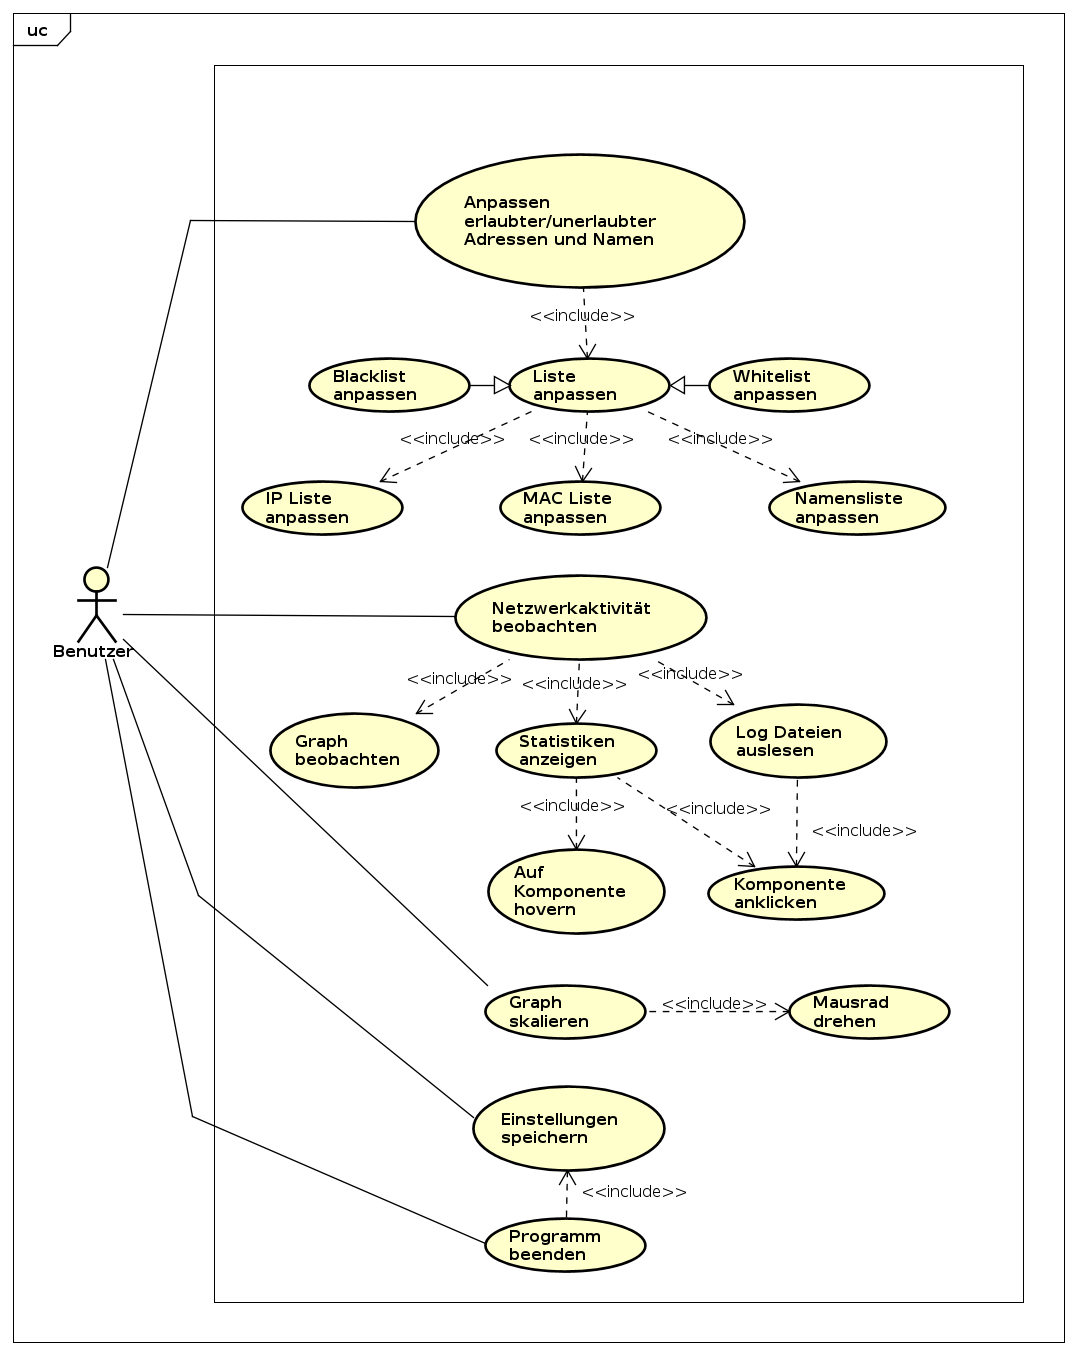
\includegraphics[width=\textwidth]{../diagrams/UC_Benutzerinteraktion.png}
    \caption{Anwendungsfalldiagramm Benutzerinteraktion}
\end{figure}

%\section{Objektmodelle}

\pagebreak
\section{Dynamische Modelle}


	\subsection{Beschreibung: Programmablauf}
	
	\begin{easylist}[enumerate]
	\ListProperties(Style2*=,Numbers=a,Numbers1=R,FinalMark1={.},FinalMark2={.},FinalMark3={.},Numbers4=l)
	
	
	& \programname wird gestartet (siehe Grafik "Starte Programm")
	
	& \programname und \sppname laufen als getrennte Prozesse
	
		&& Prozess: Wenn Snort noch nicht läuft wird Snort gestartet und sendet Paketdaten an den \programname Prozess (siehe Grafik "Pluginaktivitäten")
		
		&& Prozess: \programname startet mehrere Threads
		
			&&& Kontrollfluss:
			&&&& Prüfen auf neue Pakete
			&&&& Vorhandenes Paket wird gelesen und aus dem Puffer gelöscht
			&&&& Paket wird verarbeitet wenn vorhanden (siehe Grafik "Verarbeite Paketdaten")
			
			&&& Kontrollfluss:
			&&&& \programname reagiert und verarbeitet Benutzerinteraktion (siehe Anwendungsfälle "Benutzerinteraktion")
			
			&&& Kontrollfluss:
			&&&& \programname empfängt Paketdaten von Snort und schreibt sie in den Prozessinternen Paketpuffer
			
	& Unabhängig voneinander wird die GUI nach jeder Veränderung durch neue Paketdaten oder Benutzereingaben aktualisiert
	& Das Programm wird bei Bedarf beendet
	
	\end{easylist}

    \begin{figure}[h!]
        \hspace*{0.15cm}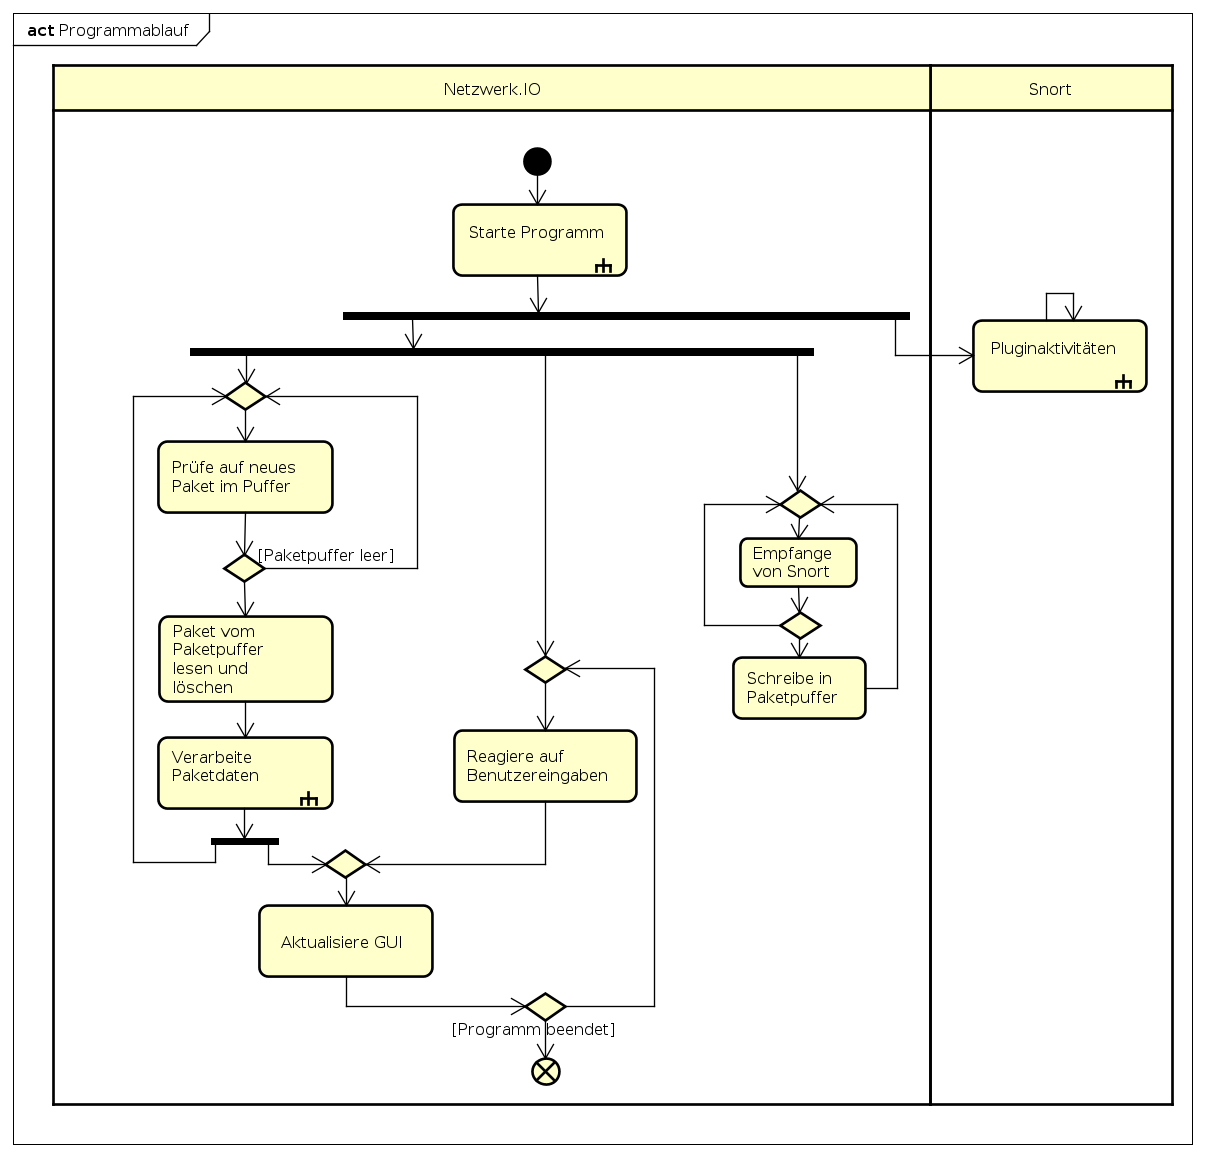
\includegraphics[width=\textwidth]{../diagrams/AD_Programmablauf}
        \caption{Aktivitätsdiagramm Programmablauf}
    \end{figure}

\pagebreak
\subsection{Beschreibung: Starte Programm}
	
	\begin{easylist}[enumerate]
	\ListProperties(Style2*=,Numbers=a,Numbers1=R,FinalMark1={.},FinalMark2={.},FinalMark3={.},Numbers4=l)
	
	
	& Initialisiere relevante Daten
	
	& Wenn Snort noch nicht läuft, frage den Benutzer ob Snort gestartet werden soll
		&& Wenn der Benutzer zustimmt wird Snort mit Plugin gestartet
		&& Wenn der Benutzer ablehnt wird Netzwerk.IO beendet
	
	& Wenn Snort schon läuft, dann Benutzer fragen ob Plugin gestartet werden soll
	    && Wenn der Benutzer zustimmt wird Snort mit dem Plugin neu geladen
	    && Wenn der Benutzer nicht zustimmt wird Netzwerk.IO beendet
	
	\end{easylist}
	
    \begin{figure}[h!]
        \centering
        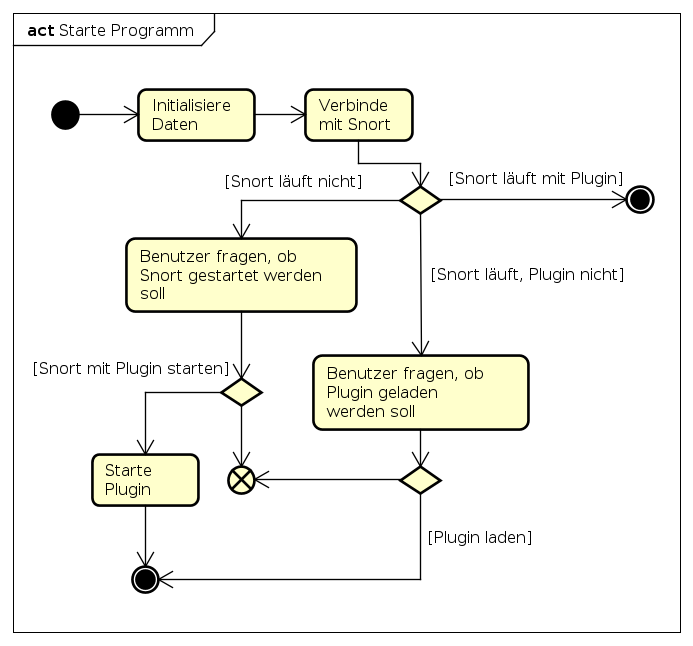
\includegraphics[width=\textwidth]{../diagrams/AD_Starte_Programm}
        \caption{Aktivitätsdiagramm Starte Programm}
    \end{figure}

\pagebreak
\subsection{Beschreibung: Pluginaktivitäten}

	\begin{easylist}[enumerate]
	\ListProperties(Style2*=,Numbers=a,FinalMark1={.},FinalMark2={.},FinalMark3={.},Numbers4=l)
	
	
	& Das Snort Plugin empfängt ein neues Paket
	& Das Paket wird dekodiert
	& Das dekodierte Paket wird auf Fehler geprüft
	    && Wenn ein Fehler gefunden wurde wird das Paket als fehlerhaft markiert
	& Das Paket wird an Netzwerk.IO weitergesendet
	& Das Paket wird für weitere Analysen auch an Snort weitergegeben
	
	\end{easylist}
	
    \begin{figure}[h!]
        \centering
        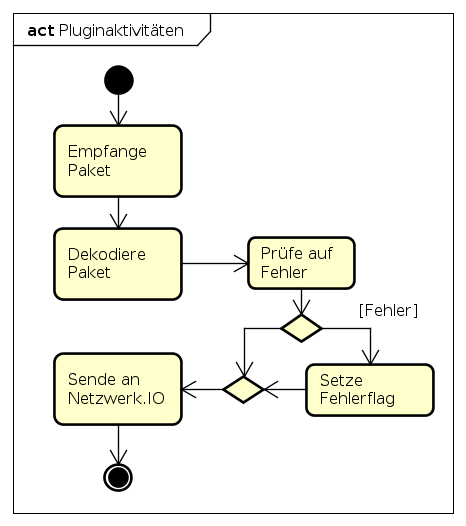
\includegraphics[width=0.5\textwidth]{../diagrams/AD_Pluginaktivitaeten}
        \caption{Aktivitätsdiagramm Pluginaktivitäten}
    \end{figure}

\pagebreak
\subsection{Beschreibung: Verarbeite Paketdaten}

	\begin{easylist}[enumerate]
	\ListProperties(Style2*=,Numbers=a,Numbers1=R,FinalMark1={.},FinalMark2={.},FinalMark3={.},Numbers4=l)
	
	
	& Das Snort Plugin empfängt ein neues Paket
	& Das Paket wird dekodiert
	& Das dekodierte Paket wird auf Fehler geprüft
	    && Wenn ein Fehler gefunden wurde wird das Paket als fehlerhaft markiert
	& Das Paket wird an Netzwerk.IO weitergesendet
	& Das Paket wird für weitere Analysen auch an Snort weitergegeben
	
	\end{easylist}
	
    \begin{figure}[h!]
        \centering
        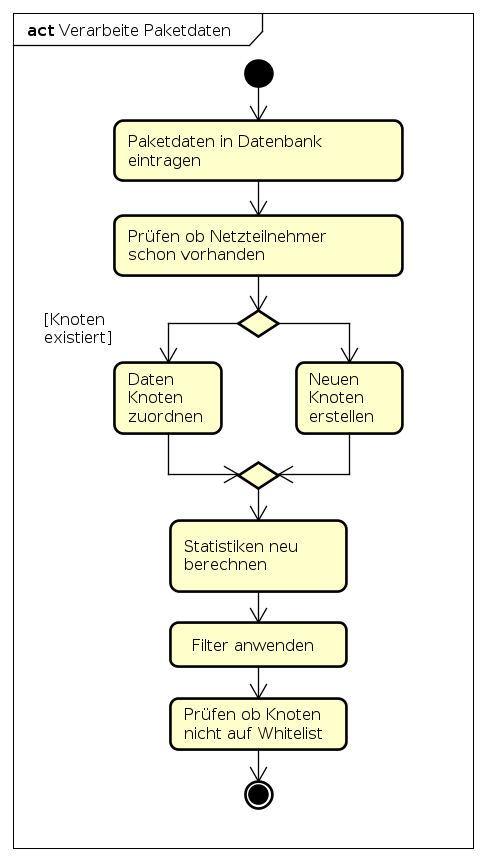
\includegraphics[width=0.5\textwidth]{../diagrams/AD_Verarbeite_Paketdaten}
        \caption{Aktivitätsdiagramm Verarbeite Paketdaten}
    \end{figure}

\chapter{\glsentrylong{gui}}

\section{Hauptfenster}
Die grafische Benutzeroberfläche ist vollbildoptimiert, lässt sich aber auch in
Fenstern skaliert anzeigen. Interaktion mit dem Benutzer findet über Hotkeys,
Mausposition und -klicks statt.
Die \gls{gui} ist standardmäßig auf Englisch.

  \begin{figure}[h!]
    \hspace*{0.15cm}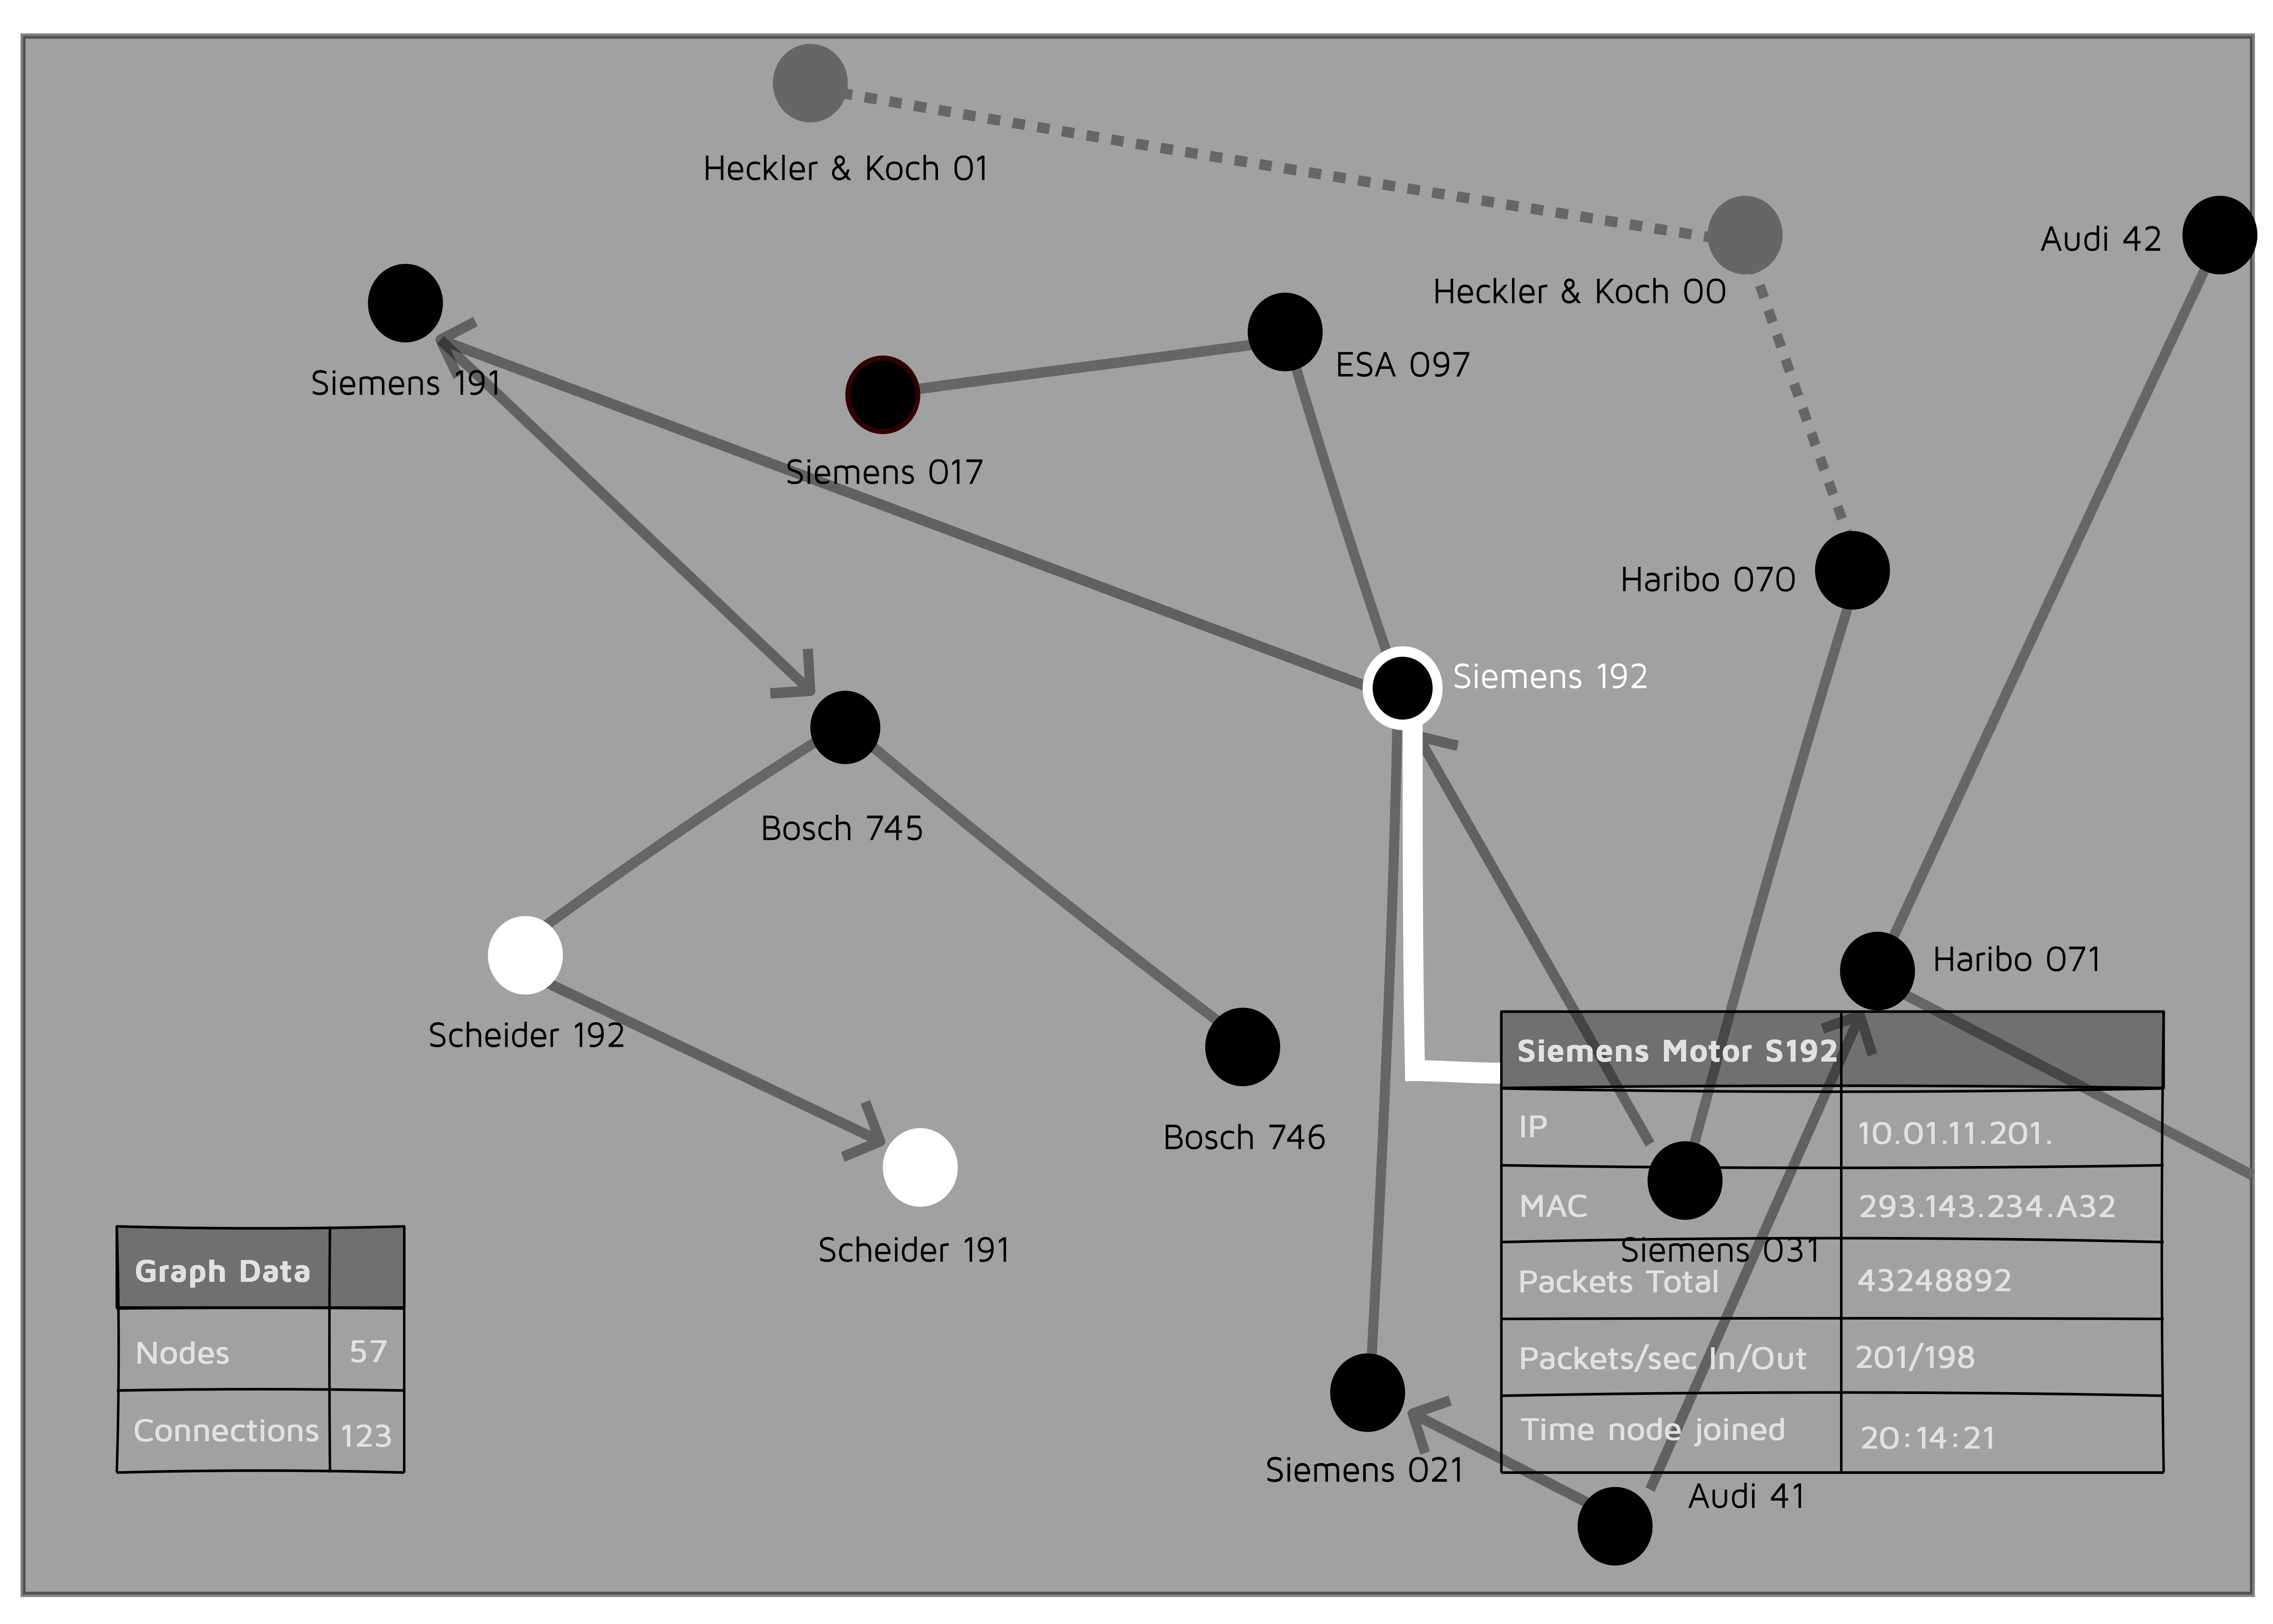
\includegraphics[scale=0.07]{./img/GUI.png}
    \caption[Die grafische Benutzeroberfläche für \gls{programname}]{Die grafische Benutzeroberfläche für \gls{programname}}
  \end{figure}

\noindent \textbf{Hintergrund:} Der Netzgraph wird im Hintergrund gezeichnet und
aktualisiert. Standardmäßig wird nur dieser dargestellt, und er ist für die
dauerhafte, interaktionslose Anzeige auf Status- oder Präsentationsdisplays
optimiert.
\\ \\
\textbf{Mittelgrund:} Einstellungsfenster, Filterfenster und optionales Statistikfenster
werden freischwebend über dem Graph dargestellt, und können verschoben und
geschlossen werden. Grundlegende Daten zum Graphen und Knoten werden an fester
Position als Overlay über dem Grahen angezeigt.
\\ \\
\textbf{Vordergrund:} Alarmfenster werden über allen anderen Fenstern angezeigt und
verschwinden nach Interaktion.

\section{Einstellungsfenster}
Das Einstellungsfenster dient zur Konfiguration der Einstellungen. Hier kann beispielsweise die Darstellung des Graphen angepasst, verschiedene
Graphalgorithmen ausgewählt werden, etc.

  \begin{figure}[h!]
    \hspace*{0.3cm}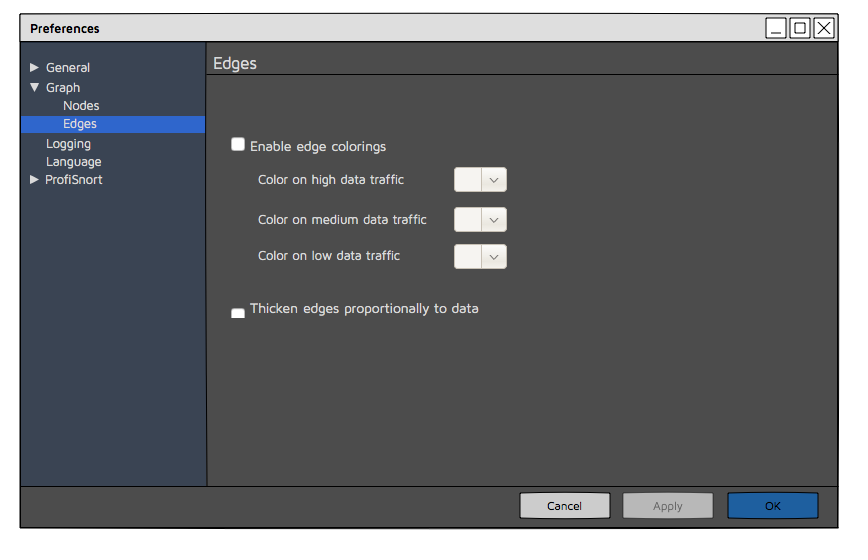
\includegraphics[scale=0.07]{./img/Preferences.png}
    \caption[Das Einstellungsfenster von \gls{programname}]{Das Einstellungsfenster von \gls{programname}}
  \end{figure}

\newpage
\section{Filterfenster}
Das Filtermenü ermöglicht dem Benutzer die Beobachtung gewünschter Knoten durch die Hervorhebung dieser. Zum Beispiel können mit dem Namensfilter alle Knoten, die einen gemeinsamen Substring enthalten, gefunden werden. In diesem Bild werden alle Siemens-Maschinen gefunden.

\begin{figure}[h!]
  \hspace*{0.2cm}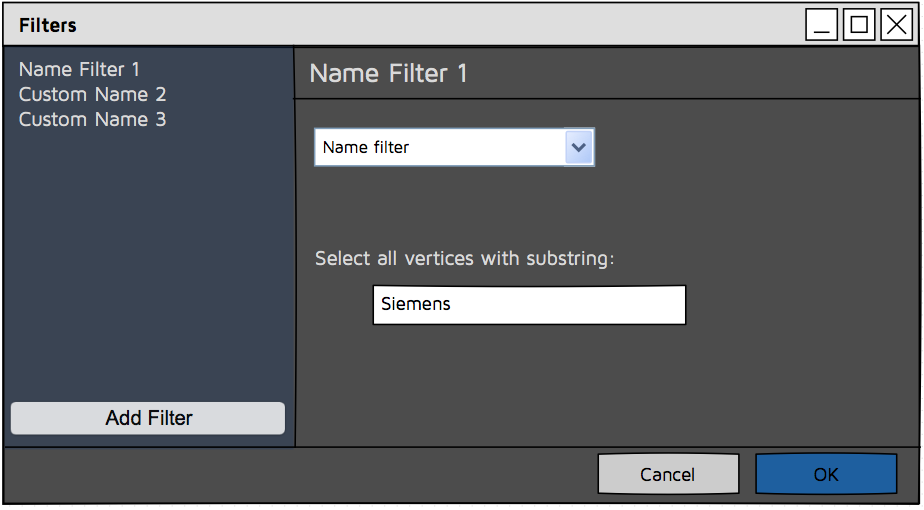
\includegraphics[scale=0.06]{./img/Filters.png}
  \caption[Das Filterfenster von \gls{programname}]{Das Filterfenster von \gls{programname}}
\end{figure}


\appendix
\chapter{Glossar}


\end{document}
